\documentclass[border=5mm]{standalone}
\usepackage{tikz}
\usetikzlibrary{cd}
\usetikzlibrary{decorations.pathmorphing,shapes,shapes.misc}
\begin{document}
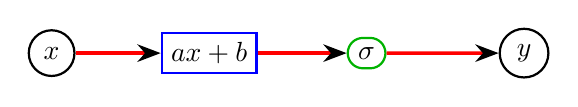
\begin{tikzpicture}
\begin{scope}[every node/.style={circle,thick,draw}]
    \node (A) at (0,0) {$x$};
    \node (D) at (6,0) {$y$};
\end{scope}
\begin{scope}[every node/.style={rectangle,thick,draw=blue}]
    \node (B) at (2,0) {$ax+b$};
\end{scope}
\begin{scope}[every node/.style={rounded rectangle,thick,draw=black!30!green}]
    \node (C) at (4,0) {$\sigma$};
\end{scope}
\begin{scope}[>={Stealth[black]},
              every edge/.style={draw=red,very thick}]
    \path [->] (A) edge node {}(B);
    \path [->] (B) edge node {}(C);
    \path [->] (C) edge node {} (D);
\end{scope}
\end{tikzpicture}
\end{document}  

%
%
%
%
%
%
%
%
%
%
%
%
%
%
%
%
%
%
%
%
%
%
%
%
%
%
%
%
















